\chapter{雜類話題II}
\section{2016年2月29日 (Instructor: Vivian)}
\subsection{立遺囑}
\mybox{\centering \textbf{注意}: 更多內容請見法律詞彙專題里的和遗嘱有关的词!}
\subsubsection*{需要掌握的單詞短語}
\begin{multicols}{2}
\begin{itemize}
  \itemsep0em
  \item 遺漏, 錯過機會: miss out
  \item 房產, 財產: property\footnote{property這個詞需要根據上下文來確定如何進行翻譯!}
  \item 資產: assets
  \item 遺產: estate
  \item 廢除: \hilight{revoke}
  \item 所有物: possessions
  \item 佔有欲: possessive
  \item 銀行存款: bank savings
  \item 自己存的退休金: \hilight{superannuation}
  \item 政府撫卹發放的養老金: pension
  \item 免除, \hilight{一筆勾銷}: be forgiven
  \item 被繼承: be inherited
  \item 健在的家庭成員: surviving family member
  \item 財產的繼承人: heirs to the property
  \item 個人債務: personal debts
  \item 值得信賴的: \hilight{trustworthy}
  \item 個人情況: personal circumstances
\end{itemize}
\end{multicols}

\subsubsection*{需要掌握的句型}
\begin{itemize}
  \itemsep0em
  \item 我想知道: I wander... (盡量少用, 這個表請求的語氣)
  \item 問區別:
  \begin{itemize}
  \itemsep0em
  	\item Is there a difference between doing A and (doing) B?
  	\item Does it make a difference if I do A or do B?
  	\item ...if one dies with or without a will?
  \end{itemize}
  \item 我的遺囑什麼時候可以生效:
  \begin{itemize}
  \itemsep0em
  	\item How can my will come into effect?
  	\item How can I make my will come into valid?
  \end{itemize}
  \item 遺囑里應該包含什麼:
  \begin{itemize}
  \itemsep0em
  	\item What should I include in my will?
  	\item What should be included in a will?
  \end{itemize}
  \item 通過遺囑檢驗獲批來生效: put into effect by a grant of probate.
  \item 以書面, 有簽字並見證的(方式): be in writing, signed and witnessed.
  \item 我對...有...的股份: of which / in which I hold...of the shares.
  \item 可能有責任承擔(法律責任): may be (held) liable for $sth.$ / to do...
  \item \hilight{貸款: take out a loan / mortgage}
  \item \hilight{資金週轉(不靈): cash / capital flow (difficulties)}
  \item 這樣是為了...: so as to do...
  \item 考慮做某事: consider doing...
  \item 對我有幫助: helpful to me
  \item 幫了我大忙了:
  \begin{itemize}
  \itemsep0em
  	\item It has helped me a lot!
  	\item It has been really helpful!
  \end{itemize}
\end{itemize}

\subsection{減肥}
\subsubsection*{需要掌握的單詞短語}
\begin{multicols}{2}
\begin{itemize}
  \itemsep0em
  \item 迭縫帶環: lap-band (surgery)\footnote{an inflatable silicone device placed around the top portion of the stomach to treat obesity, intended to slow consumption of food and thus reduce the amount of food consumed.}
  \begin{center}
  	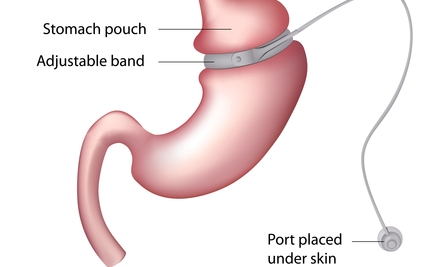
\includegraphics[scale=1.8]{pics/lap-band}
  \end{center}
  \item 脂肪抽吸手術, 抽脂術: liposuction\footnote{Areas affected can range from the abdomen, thighs and buttocks, to the neck, backs of the arms and elsewhere.}
  \item 肥胖症患者: \hilight{obese patient}
  \item 新陳代謝: \hilight{metabolism}
  \item 減肥藥: weight-loss pill
  \item 便秘的: constipated
  \item 壓迫: stain
  \item 減肥: \hilight{shape up / slim down}
  \item 高膽固醇: high \hilight{cholesterol}
  \item 高脂肪食物: \hilight{fatty foods}
  \item 心絞痛: angina
  \item 蔬菜和水果: fruit and vegetable\footnote{在英語中蔬菜水果的位置要顛倒}
\end{itemize}
\end{multicols}

\subsubsection*{需要掌握的句型}
\begin{multicols}{2}
\begin{itemize}
  \itemsep0em
  \item 我覺得疼
  \begin{itemize}
  \itemsep0em
  	\item I am \hilight{in pain}.\footnote{建議用這個, 既可以表示生理, 也可以表示心理.}
  	\item I feel pain in...
  	\item There is a pain in...
  \end{itemize}
  \item 疼得很厲害
  \begin{itemize}
  \itemsep0em
  	\item \hilight{unbearable pain}
  	\item Pain is killing me.
  \end{itemize}
  \item 促進新陳代謝: \hilight{increase metabolism}
  \item 負擔不起風險: \hilight{afford} to take such risk
  \item 一一對應: \hilight{match $sth.$ with $sth.$}
  \item 不介意做: I don't mind doing $sth.$
  \item 我只好: I have no choice but...
  \item 節食: be on a diet
\end{itemize}
\end{multicols}

\subsection{酒駕}
\subsubsection*{需要掌握的單詞短語}
\begin{multicols}{3}
\begin{itemize}
  \itemsep0em
  \item 零點零七: 0.07 / \hilight{.07}\footnote{在對話中可能.之前的零不會讀出來, 要格外注意!}
  \item 讀數: reading
  \item 初犯: \hilight{first time offender}
  \item 從輕處罰: reduce the punishment
  \item 罰我錢: fine me\footnote{fine在這裡做$v.$}
  \item 罰單: penalty notice
  \item 照章辦事: follow the rule
  \item 嚴厲: \hilight{harsh}\footnote{可以和punishment搭配}
  \item 沒氣, 沒電: flat
\end{itemize}
\end{multicols}

\subsubsection*{需要掌握的句型}
\begin{multicols}{2}
\begin{itemize}
  \itemsep0em
  \item 為什麼只攔下我呢: Why did you only stop me?
  \begin{center}
  	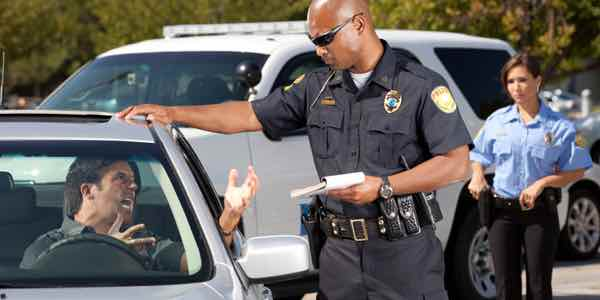
\includegraphics[scale=.4]{pics/stop-me}
  \end{center}
  \item 勸人喝酒: persuade / make $sb.$ to drink
  \item \hilight{屬於是}: falls into / within...
  \item 電池沒電了:
  \begin{itemize}
  \itemsep0em
  	\item The battery is dying.
  	\item The battery is flat.
  	\item I have run out of battery.
  \end{itemize}
\end{itemize}
\end{multicols}

\subsection{骨質疏鬆症}
\subsubsection*{需要掌握的單詞短語}
\begin{multicols}{2}
\begin{itemize}
  \itemsep0em
  \item 骨質疏鬆症: \hilight{osteoporosis}\footnote{骨質疏鬆症是一種鈣質由骨骼往血液淨移動的礦物質流失(demineralization)現象,骨質量減少,骨骼內孔隙增大,呈現中空疏鬆現象,速率取決於破骨細胞(osteoclast)和成骨細胞(osteoblast)活性的消長。此需和軟骨症(osteomalacia)有所區別,軟骨症的成因是維生素D的缺乏所導致。}
  \begin{center}
  	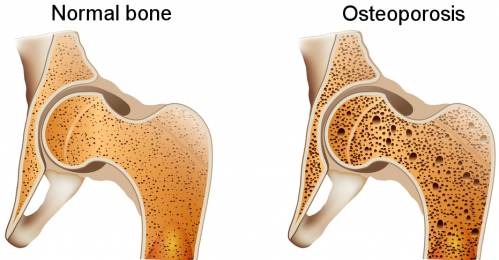
\includegraphics[scale=.5]{pics/osteoporotic}
  \end{center}
  \item 腰疼: lumbago = lower back pain
  \item 腰椎間盤: \hilight{lumbar discs}
  \item ...誘發的: \hilight{...-induced}
  \item 脊椎骨裂: fractures\footnote{這裡不要翻譯成骨折, 否則顯得很嚴重} in the spine
  \item 無症狀的: asymptomatic
  \item 止痛貼: analgesic patch
\end{itemize}
\end{multicols}

\subsubsection*{需要掌握的句型}
\begin{multicols}{2}
\begin{itemize}
  \itemsep0em
  \item 腰疼還是老樣子: lower back pain \hilight{remains the same}.
  \item 讓我做...測試: order...test for me
  \item 更容易患上...: be more susceptible to $sth.$
  \item 怎麼治: What treatments are needed?
  \item 藥一起吃: medications \hilight{mix} together.
\end{itemize}
\end{multicols}

\subsection{車禍}
\subsubsection*{需要掌握的單詞短語}
\begin{multicols}{2}
\begin{itemize}
  \itemsep0em
  \item \hilight{大清早}: early hours
  \item 左前方: \hilight{front-left}
  \item 轉彎: turn the corner
  \item 恢復知覺: \hilight{regain} your consciousness
  \item 方向盤: steering wheel
  \item 電線桿: (power) pole
  \item 行人: \hilight{pedestrians}
  \item 發生: take place
  \item (事故)現場: \hilight{scene}
  \begin{center}
  	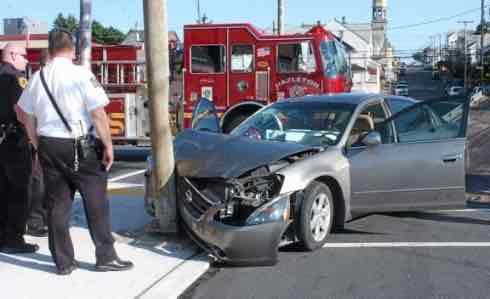
\includegraphics[scale=.45]{pics/accident-scene}
  \end{center}
  \item \hilight{證物}: exhibit
  \item 速度標誌: speed advisory sign
\end{itemize}
\end{multicols}

\subsubsection*{需要掌握的句型}
\begin{multicols}{2}
\begin{itemize}
  \itemsep0em
  \item 以...的速度行車: \hilight{drive (at the speed) of...}
  \item 沒有用: it was no use
  \item 我沒有什麼可辯解的了: I have nothing (further) to add in my defence.
\end{itemize}
\end{multicols}

\subsection{賣房}
\mybox{\centering \textbf{注意}: 更多內容請見詞彙專題里的和競拍有關的詞!}
\subsubsection*{需要掌握的單詞短語}
\begin{multicols}{2}
\begin{itemize}
  \itemsep0em
  \item 迅速上升: spike up
  \item 在你名下: \hilight{under your name}
  \item 房產證, 房契, 地契: title deed\footnote{中國的房產證可以翻譯成property ownership certificate}
  \begin{center}
  	
\includegraphics[scale=.45]{pics/deed}
  \end{center}
  \item 菜地: veggie patch
  \item 噴泉: fountain
\end{itemize}
\end{multicols}

\subsubsection*{需要掌握的句型}
\begin{multicols}{2}
\begin{itemize}
  \itemsep0em
  \item 把它賣個好價: sell it for a high price.
  \item 把...放到拍賣: \hilight{put it up for} auction.
  \item 你認為需要多久: How long do you think will it take to...?
\end{itemize}
\end{multicols}

\vspace{15mm}

\begin{center}
  \textbf{************ END OF THE DAY ************}
\end{center}
\newpage

\section{2016年3月1日 (Instructor: Chris)}
\subsection{離婚 - 財產分配}
\subsubsection*{需要掌握的單詞短語}
\begin{multicols}{2}
\begin{itemize}
  \itemsep0em
  \item 撫養權: custody / residence\footnote{現代法律中逐漸開始出現用residence代表撫養權的意思}
  \item 探視權: access
  \item 分居: separation
  \item 同屋分居: separation under the same roof
  \item 無過錯離婚: no-fault divorce
  \item 財產分配: distribution of properties
  \item 婚前協議: pre-nuptial agreement / prenup
  \item 孤島: isolated island
  \item 安慰: comfort
  \item 銀行利息: bank savings interest
  \item 牛市 / 熊市: bull / bear market
  \item 股票: share
  \item bond: (金融)債券, (租房)押金
  \item 證券: securities
  \item 福利: benefit
  \item 退休金: superannuation\footnote{月薪在\$450以下的雇主不會給交退休金}
  \item 家庭開支: family expenses
  \item 住房貸款還款費用: mortgage repayments
  \item 水電費: utilities
\end{itemize}
\end{multicols}

\subsubsection*{需要掌握的句型}
\begin{multicols}{2}
\begin{itemize}
  \itemsep0em
  \item 艱苦鬥爭: go through a tough battle
  \item 如果是你的意願: If that is your preference...
  \item 起草一個安排: draw up a (draft) schedule
\end{itemize}
\end{multicols}

\subsubsection*{注意}
\begin{itemize}
  \itemsep0em
  \item Salary代表以年或月來支付的薪水, wage代表以雙周發的錢, pay代表比較general的支付, 可以指按小時發的錢
\end{itemize}

\subsection{公共場合受傷索賠}
\subsubsection*{需要掌握的單詞短語}
\begin{multicols}{2}
\begin{itemize}
  \itemsep0em
  \item Criminal Injuries Compensation Act 1985: 1985年刑事受傷賠償法\footnote{翻譯帶有年份的法律條案時, 年份請放在最前面}
  \item amenities: 便利設施\footnote{比如房屋廣告常常會寫``close to all amenities"} / 生活情趣\footnote{比如因為殘疾會喪失很多活動的權利, 因此lose amenities of life}
  \item 索取賠償: claim compensation\footnote{在CentreLink話題中, claim常常譯為``申領"}
  \item 櫃台: counter
  \item 隊伍: queue / line
  \begin{center}
  	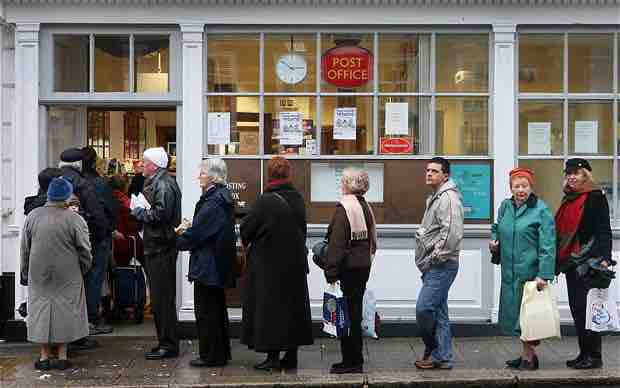
\includegraphics[scale=.38]{pics/queue}
  \end{center}
  \item 插隊: jump / cut in a queue\footnote{當你想禮貌提醒插隊的人時, 你可以先說: ``There is a queue here."}
  \item 佐證: corroborate
  \item 要求填寫的表格: prescribed form
  \item 自費的費用: out-of-pocket expenses
  \item 不值一提的事情: errands
  \item 打人身傷害的律師: personal injury lawyer
\end{itemize}
\end{multicols}

\subsubsection*{需要掌握的句型}
\begin{multicols}{2}
\begin{itemize}
  \itemsep0em
  \item 巨額賠償金: huge amount of damages
  \item 狠狠地推某人: push $sb.$ hard (不是hardly!)
  \item 疼得很厲害: ... hurts me very badly.
  \item 我的膝蓋撞到了櫃台的邊緣: My knee(s) \hilight{was} hit on the edge of the counter.
  \item 佐證你的說法: corroborate your story
  \item 最高的可賠償金額: The maximum amount of compensation payable.
  \item 這樣啊...: I see...
  \item 把醫藥費報回來: claim medical expenses back.
  \item 他們賠多少我都覺得不過分: They can't compensate me enough.
  \item 到時候...: ...by then
  \item 把違法者告上法庭: take the offender to the court.
  \item 慢慢來: take your time.
  \item 你先忙吧 / 不打擾你了: I won't hold you here\footnote{這是在中文中很常見兩個人沒話說以後結束話題的一句話, 也可以說I won't hold your any longer.}
  \item 在忙著呢: I'm just running errands.\footnote{在中文中寒暄, 當別人問你``最近乾啥呢"的時候, 你如果只想敷衍一下對方, 就可以用這句話來應付.}
\end{itemize}
\end{multicols}

\subsection{酒店投訴}
\mybox{\centering \textbf{注意}: 更多筆記被歸納到專題里的``和機場有關的詞", 請參考目錄查找!}
\subsubsection*{需要掌握的單詞短語}
\begin{multicols}{2}
\begin{itemize}
  \itemsep0em
  \item 豪華套房: deluxe suite
  \item 雙人房: en-suite
  \item 總統套房: presidential suite
  \item 過獎, 奉承: flatter
  \item (酒店的)...景房: ... view
  \item 電子轉帳: EFTPOS\footnote{electronic funds transfer at point of sale — is an electronic payment system involving electronic funds transfers based on the use of payment cards, such as debit or credit cards, at payment terminals located at points of sale.}
  \item B-Pay: 電子支付
  \item 前廳經理: front office manager.
  \item 走道: aisle
\end{itemize}
\end{multicols}

\subsubsection*{需要掌握的句型}
\begin{multicols}{2}
\begin{itemize}
  \itemsep0em
  \item 下毒: be poisoned
  \item 她好上相: This photo flattered her.
  \item 似乎崩潰了: seemed to be crashed
  \item 最開始: in the first place.
  \item 一下飛機就來了: came \hilight{right} after landing.
  \item 付款成功了: Payment was through.
  \item 為某人報復: revenge $sb.$
  \item 報復某人: revenge on $sb.$
\end{itemize}
\end{multicols}

\subsubsection*{注意}
\begin{itemize}
  \itemsep0em
  \item revenge和avenge的區別在於: revenge一般指的私下報復, 而avenge一般指的為正義而復仇
\end{itemize}

\subsection{離婚 - 分居}
\subsubsection*{需要掌握的單詞短語}
\begin{multicols}{2}
\begin{itemize}
  \itemsep0em
  \item 輓回關係: save relationship
  \item 現實的情況\footnote{原文說女主人公想離婚, 但現實情況不允許她這麼做} : actual situation
  \item 家務: domestic task
  \item 招待朋友: entertain friends
  \item 財產分配協議: property settlement agreement
\end{itemize}
\end{multicols}

\subsubsection*{需要掌握的句型}
\begin{multicols}{2}
\begin{itemize}
  \itemsep0em
  \item 過著一種非常分離的生活: lead quite separate lives
  \item 給人添麻煩: cause trouble to $sb.$ / trouble $sb.$
  \item 分居: live separately and apart
  \item 付清貸款: pay off the mortgage
  \item 注意: be mindful about\footnote{用於作為pay attention to...的替換句型}
  \item 獲准: be granted $sth.$
\end{itemize}
\end{multicols}

\subsection{離婚 - 隔壁老王被挖出}
\mybox{\centering \textbf{注意}: 請留意這篇對話的Segment 12比較牛逼, 而且Reference被閹割!}
\subsubsection*{需要掌握的單詞短語}
\begin{multicols}{2}
\begin{itemize}
  \itemsep0em
  \item 憑據: docket\footnote{有別於一般的receipt, 一般指一些類似於confirmation letter之類的憑證.}
  \item 毛皮大衣: fur coat
  \item 資產負債表: balance sheet
  \item 新娘 / 伴娘: bride / bridesmaid
  \item 新郎 / 伴郎: bridegroom / best man
  \item 婚禮誓詞: vow
  \item 婚宴: wedding banquet
  \item 人民幣: 翻譯成RMB, 不說Chinese Yuan
  \item 裸婚: marriage without property
  \item 裸考: exam without preparation
  \item 婚外情: extramarital affair
  \item 個性不合: conflict of personality
  \item 電燈泡, 小三: third wheel
  \begin{center}
  	
\includegraphics[scale=.45]{pics/third-wheel}
  \end{center}
  \item 踐行漸遠: drift apart
\end{itemize}
\end{multicols}

\subsubsection*{需要掌握的句型}
\begin{multicols}{2}
\begin{itemize}
  \itemsep0em
  \item 遲到了30分鐘: 30 mins late\footnote{永遠不要說late for 30 mins!}
  \item 我的遲到\footnote{原文說``希望我的遲到沒有給你增添麻煩"}: my lateness / my being late
  \item 我一路走過來: I walked all the way here.
  \item 把...算上: count $sth.$ in
  \item 讓某人做某事: have $sth.$ done\footnote{一般出現have sth. done都不是自己親自去做事}
  \item 我還沒來得及...: I didn't have a chance to...
  \item 安頓: settle down in...
  \item 深究內幕: dig up the detail
  \item 兩周的: fortnight
  \item 價值兩萬塊的毛皮大衣: fur coat worth 20,000 RMB.
\end{itemize}
\end{multicols}

\subsection{福利署津貼}
\subsubsection*{需要掌握的單詞短語}
\begin{multicols}{2}
\begin{itemize}
  \itemsep0em
  \item 銀行工作人員: bank staff member\footnote{``曲線救國可以說somebody works in a bank}
  \item 臨時工: casual job
  \item 零工: odd
  \item 合同工: contractor
  \item 自雇人士: self-employed
  \item 應得的錢: entitlement
  \item 收入和資產測試: income \& assets test = means test
\end{itemize}
\end{multicols}

\subsubsection*{六個補助, 兩個津貼}
\begin{itemize}
  \itemsep0em
  \item 表補助的詞: benefit, payment, assistance, subsidy, pension, support
  \item 表津貼的詞: allowance, bonus
\end{itemize}

\vspace{15mm}

\begin{center}
  \textbf{************ END OF THE DAY ************}
\end{center}
\newpage

\section{2016年3月7日 (Instructor: Vivian)}

\vspace{15mm}
\begin{center}
  \textbf{************ Stay tuned ... ************}
\end{center}